% Class
\documentclass{beamer}

% Base
\usepackage[british]{babel}
\usepackage[T1]{fontenc} 
\usepackage[utf8]{inputenc} 

\usepackage{color, colortbl}
\usepackage{fancyvrb}
\usepackage{enumitem}
\usepackage{multicol}
\usepackage{multirow}
\usepackage{xcolor}
%\usepackage{algpseudocode}
\usepackage{array}

% Règle les conflits beamer/enumitem
\setitemize{label=\usebeamerfont*{itemize item}
\usebeamercolor[fg]{itemize item}
\usebeamertemplate{itemize item}}
  
% Thème
\usetheme{Antibes}

% Titre
\title{Communication LoRa avec les Motes Wyres}

% Dossier images
\graphicspath{{imgs/}}

% Auteur, lieu, date
\author{
\includegraphics[scale=0.3]{univ.png} \\~ \\ ~ Alexandre SAHUC\\~ Erwan CROZE}

\institute{Université Joseph Fourier \newline M2M}
\date{\today}

% Puce triangle
\setbeamertemplate{itemize item}[triangle]

% A chaque changement de section, affichage de la section dans une diapo
\AtBeginSection[ ]
{
	\begin{frame}
 		\tableofcontents[currentsection,hideothersubsections]
 	\end{frame}
}

% Marges du diapo
\setbeamersize{text margin left=0.8cm, text margin right=0.8cm}

% Numéros de pages
\defbeamertemplate*{footline}{shadow theme}
{%
	\leavevmode%
	\hbox{\begin{beamercolorbox}[wd=1.0\paperwidth,ht=2.5ex,dp=1.125ex,leftskip=.3cm plus1fil,rightskip=.3cm]{author in head/foot}%
    	\usebeamerfont{author in head/foot}\insertframenumber\,/\,\inserttotalframenumber\hfill
	\end{beamercolorbox}%
}%
	\vskip0pt%
}

\newcolumntype{M}[1]{>{\raggedright}m{#1}}
\newcolumntype{C}[1]{>{\centering\arraybackslash}m{#1}}

\begin{document}

% Diapo de présentation
\begin{frame}
	\titlepage
\end{frame}

\section{Presentation}
\subsection{Projet}
\begin{frame}
  	\begin{block}{Principe}
  		Utiliser des émetteurs LoRa pour communiquer avec une gateway qui enverrait les informations sur un serveur où l'on pourrait les analyser.
	\end{block}
	
	\begin{exampleblock}{Matériel}
		\begin{itemize}
			\item Deux Motes Wyres (emetteur/recepteur)
			\item carte SX1301 IMST iC880A (Gateway)
			\item Raspberry PI 
		\end{itemize}
	\end{exampleblock}
\end{frame}

\section{LoRa}
\begin{frame}
	\begin{block}{Description}
		LoRa permet la communication par radio à bas débit entre des objets.
		LoRaWan est une extension de LoRa.
		\center
		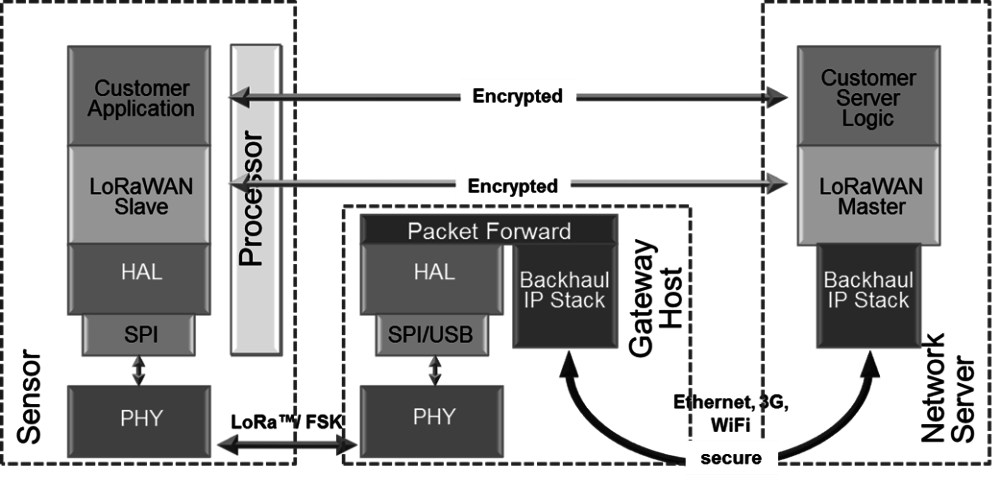
\includegraphics[scale=0.5]{LoRa-network.png}
	\end{block}
\end{frame}

\section{Client}
\begin{frame}
	\begin{block}{Programmes Motes}
		\begin{itemize}
			\item serialcom
				\begin{itemize}
					\item Permet d'envoyer des commandes au Motes (une ou plusieurs commandes)
				\end{itemize}
			\item sensor
				\begin{itemize}
					\item Récupère et envoie périodiquement la moyenne de la température CPU sur le réseau LoRawan
				\end{itemize}
		\end{itemize}
	\end{block}
\end{frame}

\begin{frame}
	\begin{block}{Programmes Gateway}
		\begin{itemize}
			\item packet\_forwarder
			\begin{itemize}
				\item Ecoute sur certaines fréquences et transfert à un serveur les messages reçus
			\end{itemize}
		\end{itemize}
	\end{block}
\end{frame}

\section{Serveur}
\begin{frame}{Architecture}
	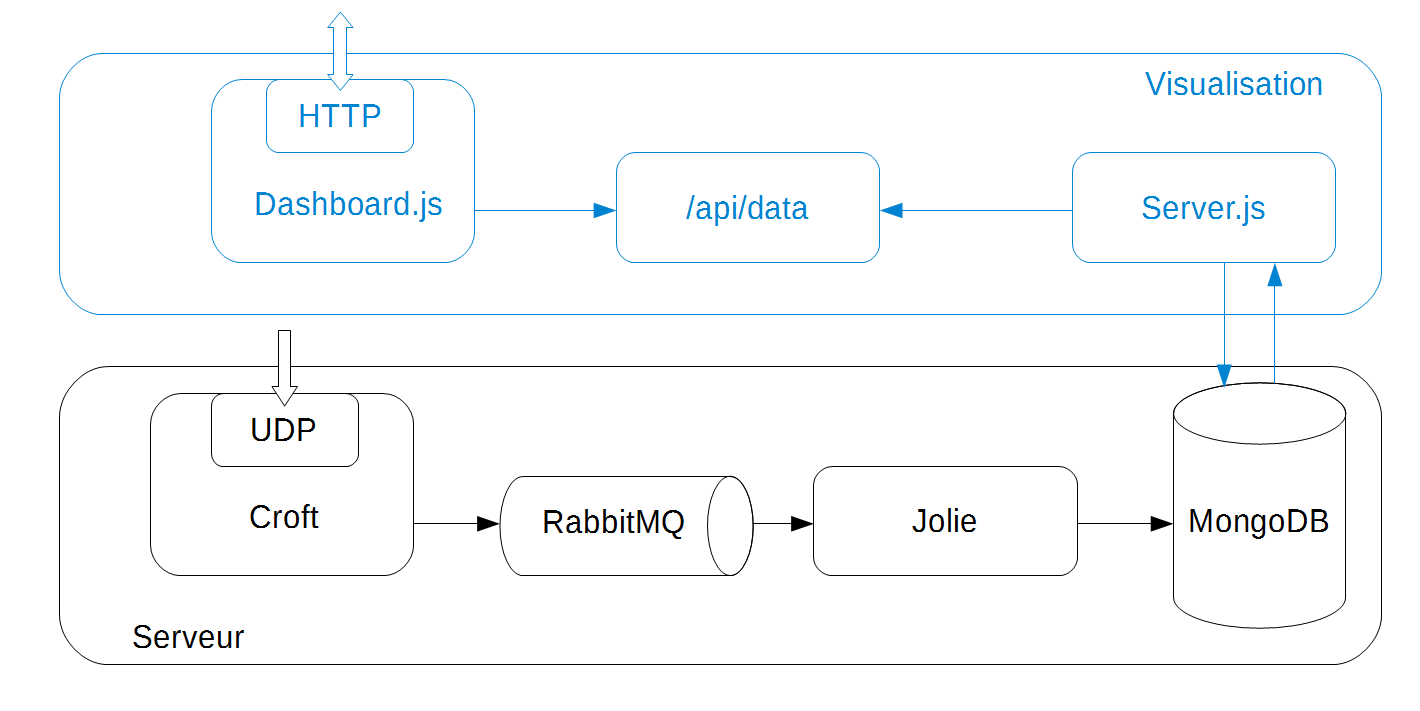
\includegraphics[scale=0.3]{M2M.png}
\end{frame}

\section{Conclusion}
\begin{frame}
	\begin{block}{Problèmes rencontrés}
		\begin{itemize}
			\item Les Motes Wyres ne peuvent pas communiquer en point à point
			\item Documentation des Motes Wyres pas à jour
			\item Impossibilité de déchiffrer les données à la réception
		\end{itemize}
	\end{block}
\end{frame}
\end{document}



















